\section{Recipe features}
\label{sec:features}

Over time, several advanced features in the recipes have been developed following user feedback.
In this section, I explain the problems they tackle and provide code examples for each one.

\subsection{Lowering effective false positives}
\label{sec:efp}
It is important to choose the right error level for the developer to pay attention to the markings, but also not to overwhelm them with markings to the point that they start to ignore them.
Since the recipes can be created by anyone in the team, they should not be too obtrusive.
To a recipe-writer, a false positive is an incorrect marking of code that is not violating a coding guideline.
However, to a developer, a false positive is any code marking that they do not intend to fix and ignore instead~\cite{ayewah2007evaluating}.
A false positive from the perspective of the developer is also called an \gls{efp}~\cite{sadowski2015tricorder}.
To ensure the usability of the tool, the \gls{efp} rate should be sufficiently low~\cite{sadowski2015tricorder,johnson2013don}.

To demonstrate \glspl{efp} we take a look at \gls{os} Command injection.
One of the \glspl{api} that is banned in the \gls{owasp} \gls{esapi} guidelines is \texttt{Runtime.exec}.
This \gls{api} is used to execute \gls{os} commands in Java programs.
When user input is added to this command, \gls{os} command injection is possible and the attacker can gain access to the underlying \gls{os}.
Using this information it is possible to create a recipe that marks all uses of the \texttt{Runtime.exec} method.
While this is a good coding guideline, a security conscious developer recognizes that the method needs user input before it can lead to \gls{os} command injection.
In rare occasions an \gls{os} command might be necessary for functionality and perfectly valid and secure.
For example, launching another software product can be done securely as long as the command is hard-coded.
An example of insecure usage of the \texttt{Runtime.exec} method can be found in Listing~\ref{lst:oscommand1}, examples of secure usage in Listings~\ref{lst:oscommand2}~and~\ref{lst:oscommand3}.
The two secure examples are still violations of the above coding guideline, and they get flagged.
An experienced developer has no intent to fix them, meaning they are two cases of \glspl{efp}.
Notice how this \gls{efp} depends on the knowledge and skill of the developer, meaning that it might be beneficial to adjust the feedback of the tool for individual developers, as explained in the perspectives in Section~\ref{sec:sensei-perspectives}.
%A similar example leading to \glspl{efp} is when hard-coded \gls{sql} queries are created without using parameterized queries.
%These queries would violate a guideline enforcing parameterized queries, but they would not be insecure, not even when this function is reused from a different context in the future.

In order to keep the \gls{efp} rate sufficiently low, we have introduced the concept of \emph{trusted input}.
Hard-coded input is automatically trusted, since a user can not influence it, and hence it can not lead to a vulnerability.
However, function parameters and variables from other origins are considered untrusted by default.
This is still in line with the philosophy to protect methods from future use, where we want to flag violations that can one day lead to vulnerabilities.
The requirement in recipes of untrusted input can be added to arguments, this can be done using the \gls{yaml} syntax or by using the \gls{gui} as shown in Figure~\ref{fig:recipegui}. 
The next step is to define trusted sources. This also avoids the \gls{efp} in Listing~\ref{lst:oscommand3}. The resulting recipe can be seen in Listing~\ref{lst:yamlrecipe}.

\begin{minipage}[t]{0.9\linewidth}
%\vspace{-0.4 cm}
\begin{lstlisting}[language={Java},caption={if the \texttt{command} variable contains unsanitized user input, this function is vulnerable to \gls{os} command injection.},label={lst:oscommand1},abovecaptionskip=-0.0pt,xleftmargin=15pt]
public void executeCommand(String command){
    Runtime r = Runtime.getRuntime();
    r.exec(command);
}
\end{lstlisting}
%\vspace{-0.3cm}
\begin{lstlisting}[language={Java},caption={Using a hard-coded command avoids the possibility that the variable will ever contain unsanitized user input.},label={lst:oscommand2},abovecaptionskip=-0.0pt,xleftmargin=15pt]
public void executeCommand(){
    Runtime r = Runtime.getRuntime();
    r.exec("explorer.exe");
}
\end{lstlisting}

\begin{lstlisting}[language={Java},caption={This code fragment is secure if the \texttt{getSafeCommand} method can be trusted to never return variables containing unsanitized user input.},label={lst:oscommand3},abovecaptionskip=-0.0pt,xleftmargin=15pt]
public void executeCommand(){
    Runtime r = Runtime.getRuntime();
    String command = getSafeCommand();
    r.exec(command);
}
\end{lstlisting}

\begin{lstlisting}[language={yaml},caption={This recipe trigger requires the argument of an \texttt{exec} methodcall to contain untrusted input before it will mark the methodcall. It also specifies the methodcall \texttt{getSafeCommand} as a trusted source of input.},label={lst:yamlrecipe},xleftmargin=15pt]
search:
  methodcall:
    name: "exec"
    type: "java.lang.Runtime"
    args:
      1:
        type: "java.lang.String"
        containsUntrustedInput: true
        trustedSources:
        - methodcall:
            name: "getSafeCommand"
\end{lstlisting}
\end{minipage}
%\vspace{-.3cm}

\begin{figure}[t]
  \centering
  %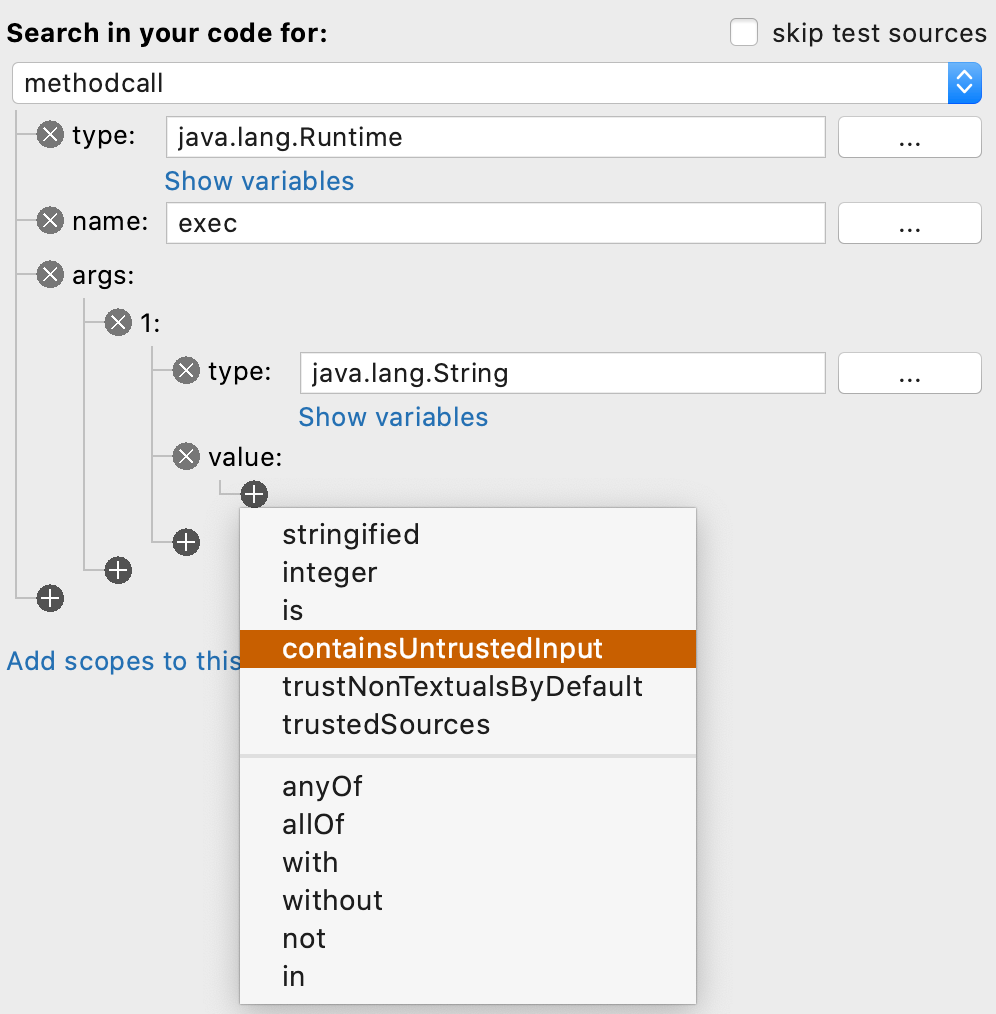
\includegraphics[width=\textwidth]{rulegui2.png}
  \includegraphics[width=0.85\textwidth,page=9]{04-tools/figures/figures2.pdf}
  \caption[\Gls{gui} to add the requirement of untrusted input.]{It is possible to add requirements like untrusted input or an in-clause through the \gls{gui}.}
  \label{fig:recipegui}
\end{figure}

Another way to allow recipe-writers to create more targeted recipes and to keep the \gls{efp} rate low, is to provide \emph{trigger scopes}.
Trigger scopes can be added by using the \texttt{in} keyword in the \gls{yaml} syntax, or by using the \gls{gui} as shown in Figure~\ref{fig:recipegui}.
The in-clause can define restraints on the context.
This makes it possible to create a recipe that prevents the usage of \texttt{Runtime.exec} except in a class with name \texttt{AppLauncher}.
Scopes like this can also help with performance, i.e., meeting the real-time checking requirement, since recipes that are out of scope can be skipped during analysis.

In the old editor, rather than \emph{trigger} scopes, \emph{recipe} scopes were a property of the entire recipe.
They were added by selecting the type of scope and filling in some fields.
By migrating these scopes to the \gls{yaml} syntax, the scoping of recipes becomes more flexible.
The recipe scopes that can be migrated to trigger scopes are the class scope, method scope, file scope, Android context scope, and Android build property scope.
Descriptions of these scopes can be found in Appendix~\ref{app:recipe-scopes}.

There are two more recipe scopes, for which migration to trigger scopes is not useful.
The \emph{project scope} allows us to enable or disable recipes based on the name of the project.
This is useful when different cookbooks are required for each project in a company.
This scope is no longer needed since we now allow cookbooks to be stored in the project, which is a lot more convenient then adding a scope to each recipe separately.
The \emph{library scope} can be used to enable recipes based on the presence of a library.
This way we can disable a recipe if the fix uses a library that is not used in the project.
Since this scope is created for the fix of the recipe and not the trigger, it cannot be added to the \gls{yaml} syntax and remains a property of the entire recipe.
In the future it could be useful to add scopes to quick-fixes, so that a recipe can provide different fixes depending on the presence of a library.

\subsection{Support for libraries}
Often quick-fixes are small code changes, such as adding a preceding method call or changing a parameter, but sometimes they involve more elaborate pieces of code.
An example for this is adding a cookie to a \gls{http} request.
Before adding the cookie, it needs to be properly configured.
Insecure and secure code examples are shown in Listings~\ref{lst:cookie1} and~\ref{lst:cookie2}, respectively.

\begin{lstlisting}[float,language={Java},caption={This cookie is not configured before it is added to the response, as a result this code fragment is insecure.}, float,label={lst:cookie1},abovecaptionskip=-0.0pt]
Cookie myCookie = new Cookie("secure", "success");
response.addCookie(myCookie);
\end{lstlisting}

\begin{lstlisting}[language={Java},caption={Several configuration options are added to narrow the scope that the cookie can be used, and to ensure it is not sent over plaintext.}, float,label={lst:cookie2},abovecaptionskip=-0.0pt]
Cookie myCookie = new Cookie("secure", "success");
myCookie.setSecure(true);
myCookie.setHttpOnly(true);
myCookie.setDomain("sub.domain.scw.com");
myCookie.setPath("more/narrow/path");
response.addCookie(myCookie);
\end{lstlisting}

If this fix is applied at multiple locations in a project, it can result in code bloat.
It might then be better for the company to provide a method that replaces the original \texttt{addCookie} method.
In this method the cookies can be first configured properly before calling the original \texttt{addCookie} method.
Such a replacement wrapper method is shown in Listing~\ref{lst:cookie3}.
The new guideline for cookies is then to replace the \texttt{addCookie} method with the \texttt{safeAddCookie}, as shown in Listing~\ref{lst:cookie4}.
The creation of such a wrapper library is strongly recommended by the paved path methodology, as the resulting guidelines are easy to understand for developers.
At the same time any security bugs are confined to the \textit{implementation} of the wrapper library, and no new bugs can be introduced by \textit{using} the wrapper library. This makes the job of the security team easier as well.

\begin{lstlisting}[language={Java},caption={A wrapper library can be created to avoid code reuse and to improve clarity of the guidelines for the developer.}, float,label={lst:cookie3},abovecaptionskip=-0.0pt] 
public void safeAddCookie(Cookie myCookie, HttpServletResponse response){
    myCookie.setSecure(true);
    myCookie.setHttpOnly(true);
    myCookie.setDomain("sub.domain.scw.com");
    myCookie.setPath("more/narrow/path");
    response.addCookie(myCookie);
}
\end{lstlisting}

\begin{lstlisting}[language={Java},caption={Migrating to the wrapper library consists of replacing the original methodcall with one from the library.},float,label={lst:cookie4},abovecaptionskip=-0.0pt]
Cookie myCookie = new Cookie("secure", "success");
safeAddCookie(myCookie, response);
\end{lstlisting}

The first example, where the cookie is configured properly, is a \emph{library usage recipe}.
This type of recipe provides guidance on using a library correctly.
The trigger of the recipe is on \glspl{api} from the library.
Code fragments are refactored without involving additional libraries, only libraries that are also used in the trigger.

The second example, where the insecure code is replaced with \gls{api} calls from a different library, is a \emph{library adoption recipe}.
Instead of providing guidance on the correct usage of the \glspl{api}, such recipes promote the adoption of a new library.
This type of recipe has a trigger in one library but their fix uses a different library.

As a proof of concept for library adoption recipes, support has been developed for the \gls{owasp} \gls{esapi} library.
Among others, the \gls{owasp} \gls{esapi} contains replacement methods for commonly used insecure \gls{jdk} methods, the so-called \gls{owasp} \gls{esapi} banned \glspl{api}\footnote{\url{https://www.owasp.org/index.php/ESAPI\_Secure\_Coding\_Guideline}}.
To support the \gls{owasp} \gls{esapi} in companies that adopt it, a recipe set was created to enforce the replacement of the banned \glspl{api} with their alternatives from the \gls{owasp} \gls{esapi}.
Feedback from these companies showed that this set of library adoption recipes was intuitive and easy to use for developers.
Importantly, it increased the speed of the library's adoption.

Library usage recipes are generally applicable to codebases because the trigger and fix of these recipes use \glspl{api} from the same library, thus ensuring that the recipes never mark any code when the fix is unavailable.
The trigger and fix for library adoption recipes depend on different libraries.
This implies that an applied quick-fix can result in the use of unavailable \glspl{api}. 

Library scopes can be used for this purpose.
When the library used in the quick-fix serves as a scope of a recipe, it will not mark any code if the library is unavailable.

\subsection{Support for detecting design flaws}
As discussed before, coding guidelines are enforced through mostly local analyses.
This allows Sensei to intervene earlier in the development process and makes it possible to perform the analyses in real time while the developer is typing.
For this reason the focus of the approach is mostly on implementation bugs.
Detecting design flaws in the application code (rather than in the \glspl{api} it relies on) is typically harder.
Still, we have learned that various flaws can be tackled through the use of configuration files and the previously described trigger and recipe scopes.

An example of a flaw that is difficult to detect with local analyses is excessive security logging.
It is crucial to log important security events, but too much logging can make it difficult or impossible to locate certain events.
While enforcing guidelines can help with logging securely (e.g., not logging sensitive data, not logging unsanitized input, logging in proper format) it is difficult to monitor the frequency of the logging through local analyses.
Other examples are the use of transport layer security, or whether authorization is needed or not.

One scenario that, to the contrary, enables us to detect some design flaws, is when popular frameworks are used to implement security features.
For example, enforcing the use of transport layer security in an Android app is as simple as adding a line to the Android manifest about clear text traffic.
This can be seen in Listing~\ref{lst:manifest}, line 3.

\begin{lstlisting}[language={XML},caption={When the attribute \texttt{usesCleartextTraffic} is added to the Android manifest with value \texttt{false}, the Android \gls{os} will ensure that transport layer security is used for the communication with this application.},float,label={lst:manifest},abovecaptionskip=-0.5pt]
<application
     android:label="@string/app_name"
     android:usesCleartextTraffic="false">
\end{lstlisting}

Another example is the use of encryption.
It is trivial to detect if a deprecated encryption algorithm is used by means of a known \gls{api}, but it is harder to detect the absence of encryption through local analyses.
One interesting class of mistakes that we observed was developers XOR’ing data, or encoding data, rather than encrypting it.
As a solution, a coding guideline can be created that requires functions whose name contains “encrypt” to perform encryption through some of their approved \gls{api} methods.
If such a function \emph{only} performs encoding or XOR operations, it implies that the required \gls{api} calls are missing.
In that case the tool suggests quick-fixes that insert the necessary \gls{api} calls.
These quick-fixes are only partial fixes: They inject code that invokes encryption routines on an unspecified string or byte array.
It is then still up to the developer to remove the XOR operations and fill in the correct string or array identifier.
This emphasizes again why it is beneficial to provide fixes in the \gls{ide} during development time.
When this recipe is used during the development of a new method, the developer starts by creating a function declaration.
When a function exists with ``encrypt" in the name and an empty body, this is marked, as the required \gls{api} calls are missing.
The fix then inserts the required \gls{api} calls, leading to comfortable and intuitive security help for the developer.
This recipe is a good example to demonstrate the paved path methodology.
It guides the developer along a predetermined path laid out for them to implement encryption securely.

We have also improved context-awareness to detect flaws by adding more recipe scopes.
One such example is the Android \emph{context scope}.
As explained earlier, in the Android manifest a developer can configure capabilities of components such as activities and broadcast receivers regarding their communication towards the \gls{os}.
They can listen to any other application, only to authorized applications, or only to the own application.
The Android context scope allows us to enable recipes based on the configuration of the relevant component, so that we can enforce different recipes for different levels of exposure.
Such a recipe can allow communication of sensitive information between classes that are configured as private components, but not between other classes.

\subsection{Testing recipes}
%\todo[inline]{Add example of indexing of arguments and quickfixes}
Testing custom recipes is a challenge.
When new recipes are created, the recipe-writers first have to test the behaviour of the recipe manually.
They develop a few code fragments they expect to be marked, as well as some that should not be marked by the recipe.
They then apply the transformations and manually inspect the resulting changes.
The recipe wizard helps speed up these tasks by providing preview panels during recipe creation.
A recipe-writer at a company, however, cannot be asked to perform the manual checks again every time they install updates to our plugin (including its underlying analyses) or to the \gls{ide} itself.
Such updates always risk altering the outcome of a recipe.
Instead automated testing is needed.

Such testing is available to the plugin developers at \gls{scw}.
They have sufficient capabilities to automate unit tests that verify the behavior of the analyses.
To do this, they also create a few demo recipes and test the behavior of these recipes.
Since they have access to the code of the plugin, they can simply write unit tests and (directly) call internal plugin and exported \gls{ide} methods to test the markings and transformations and to compare them to the expected results.
In other words, they can write code snippets that verify whether or not updates to tools alter the deployment of existing recipes.
Such testing is unavailable to the custom recipe-writers in a company, however, which do not have access to, and definitely do not want to learn, the internal plugin \glspl{api}.  

A better testing framework is hence required, such that the recipe-writers in companies can indicate the expected outcomes of every recipe they wrote on a number of code samples.. 
If we allow recipe-writers to define tests in the plugin itself, and store them in the cookbooks, these tests can automatically be performed when loading a new cookbook and after every \gls{ide} and plugin update.
We can then notify the user when one of the recipes is no longer working as expected.

In the new recipe wizard it could be possible for the recipe-writer to select one or more of the examples that are marked in the preview panels and allow these examples to be used as the recipe tests.
This way the recipe-writers are creating tests for their recipes with nearly no additional cognitive effort.
However, this comes with the problem that (possibly confidential) code of the client is then stored in these recipe tests.
At this point in time, implementing the necessary support for recipe-writer defined tests remains future work.

%\subsection{Code generators}
%When developers use the plugin for a while they get used to certain fixes being available. They know that if they write an insecure SQL query, the quick fix is able to secure it for them. This results in developers purposefully making mistakes because it takes less effort to let the plugin fix it. In order to improve this process we have created code generators. Generators are secure code fragments that can be inserted with a shortcut. Code generators are developed by the recipe-writer, and rolled out to the developer, just like the recipes. They consist of a name and the inserted code. In order for generators to be successful, they need to adapt the generated code to the context, similarly to how the quick fixes adapt when they are applied (relying on the use of the template language in their specification). From our experience with early versions of the generators, where the inserted code was not adapted to the context, e.g., to reuse the variable names occurring in the original code, we learned that that such a lack of adaptivity was a blocker for the take up by developers. More adaptive generators have not been implemented so far, validating whether this will improve their use remains future work.